% ---------------------------------------------------------------
% TO COMPILE USE: pdflatex -shell-escape -jobname report *.tex
% ---------------------------------------------------------------

\documentclass[12pt,a4paper]{article}

% ---------------------------------------------------------------
% ALL PACKAGES
% ---------------------------------------------------------------
\usepackage[left=3cm,right=2.5cm,top=3cm,bottom=2.5cm]{geometry}
\usepackage[utf8]{inputenc}
\usepackage[portuguese]{babel}
\usepackage{indentfirst}
\usepackage{graphicx}
\usepackage{hyperref}
\usepackage{caption}
\usepackage{subcaption}
\usepackage{listings}
\usepackage{enumitem}
\usepackage{float}
\usepackage{color}
\usepackage{booktabs}
\usepackage[dvipsnames,table,xcdraw]{xcolor}
\usepackage{url}
\usepackage{amsmath}
\usepackage{mathabx}
\usepackage{mathtools}
\usepackage{outlines}
\usepackage[normalem]{ulem}

\usepackage{minted} %for code template
\usemintedstyle{friendly}
\definecolor{bg}{rgb}{0.96,0.96,0.96}





\begin{document}
% ---------------------------------------------------------------
% FIRST PAGE
% ---------------------------------------------------------------
\begin{titlepage}
    \centering
    \begin{figure}[H]
        \centering
        
\includegraphics[scale=2.2]{images/logo_um.jpg}
    \end{figure}
    {\huge\bfseries Universidade do Minho \par}
    \vspace{0.5cm}
    {\large Mestrado Integrado em Engenharia Informática \par}
    \vspace{2cm}
    {\Large \emph{System Deployment and Benchmarking} \par}
    \vspace{2cm}
    {\Large Fase 1 \par}
    \vspace{0.2cm}
    {\Large\bfseries \emph{Deployment} da aplicação \emph{GitLab} \par}
    \begin{figure}[H]
        \centering
        
\includegraphics[scale=0.5]{images/gitlab_logo.png}
    \end{figure}
    \vspace{2.5cm}
    {\Large Grupo 4 \par}
     \vspace{0.5cm}
    {\Large\itshape João Alves (A77070)\par}
    {\Large\itshape Gonçalo Raposo (A77211)\par}
    {\Large\itshape Alexandre Dias (A78425)\par}
    {\Large\itshape Hugo Oliveira (A78565)\par}
    \vfill
    {\large \today\par}
    \centering
\end{titlepage}




% ---------------------------------------------------------------
% ABSTRACT
% ---------------------------------------------------------------
\vspace*{\fill}
\begin{abstract}
Paragraph 1.

Paragraph 2.

Paragraph 3.
\end{abstract}
\vspace*{\fill}
\thispagestyle{empty}




% ---------------------------------------------------------------
% TABLE OF CONTENTS
% ---------------------------------------------------------------
\clearpage
\tableofcontents
\listoffigures
\clearpage




% ---------------------------------------------------------------
% INTRODUCTION
% ---------------------------------------------------------------
\setcounter{page}{1}
\section{Introdução}
Hoje em dia, grande parte da população prescinde de algum do seu tempo em deslocações, para, e dos seus locais de trabalho, e espera-se que permaneçam no seu escritório, cumprindo assim os seus horários estabelecidos nos contratos. No entanto, apesar de já existirem várias empresas que são remote-friendly, o \emph{GitLab}, adotou uma ideia bastante diferente na sua organização, e abandonou o conceito de escritório físico permanentemente.

Neste trabalho serão analisados os componentes constituintes do \emph{GitLab}, bem como a sua estrutura. Serão analisados os componentes críticos para o desempenho da aplicação.






% ---------------------------------------------------------------
% CONTENT
% ---------------------------------------------------------------
\newpage
\section{\emph{GitLab}}
Antes de podermos descrever toda a arquitetura e funcionamento do \emph{GitLab}, é necessário perceber o que é o \emph{\textbf{git}}.

\subsection{O que é o \emph{git}?}
O \emph{git} é um sistema \emph{open source} que permite controlar versões de ficheiros de um projecto de uma forma rápida e eficaz.

O uso de um sistema como este, permite, em projetos que possam envolver vários contribuidores, criar e editar ficheiros em simultâneo, bem como retroceder a versões mais antigas destes. Assim, existe a possibilidade de analisarmos toda a evolução de um projecto.

\subsection{O que é o \emph{GitLab}?}
O \textbf{\emph{GitLab}} é uma plataforma grátis que permite hospedar projectos em servidores locais ou remotos, utilizando o \textbf{\emph{git}} para fazer o controlo de versões. O \emph{GitLab} é um concorrente \emph{open source} direto aos serviços \emph{GitHub} e \emph{Bitbucket}.

Para além desta sua principal funcionalidade, a empresa \emph{GitLab} disponibiliza o código da sua aplicação para que qualquer utilizador possa a usar livremente num outro ambiente. Recentemente, foi disponibilizado uma imagem \emph{Docker} que permite instalar e correr o \emph{GitLab} facilmente. Para uma utilização que permita uma alta disponibilidade da aplicação, é necessário alterar e configurar os diferentes componentes da \emph{stack} aplicacional do \emph{GitLab}.

\subsection{\emph{GitLab Software Delivery}}
Existem atualmente dois tipos de distribuição do \emph{GitLab}, a versão CE (\emph{Community Edition}) e a versão EE (\emph{Enterprise Edition}).

\begin{itemize}
    \item \textbf{\emph{Community Edition}}: é uma versão \emph{open source} onde não apoio de uma qualquer empresa no processo de \emph{delivery} ou \emph{deployment}. Apresenta funcionalidades reduzidas.
    \item \textbf{\emph{Enterprise Edition}}: ao contrários da versão anterior, esta inclui vários serviços para além dos incluidos na versão CE, entre estes, destacamos o suporte técnico especializado 24/7, a gestão adicional de servidores, \emph{performance} e segurança, ferramentas de estatística. Esta versão apresenta diferentes preçários mensais.
\end{itemize}












% ---------------------------------------------------------------
\newpage
\section{Arquitetura do \emph{GitLab}}\label{arq}

A alta \textbf{disponibilidade} e \textbf{escabilidade} são, hoje em dia, condições importantes e obrigatórias em qualquer aplicação. Se estes requisitos não são cumpridos, os utilizadores podem querer migrar para outra aplicação idêntica.

Um dos principais aspetos para a alta disponibilidade, consiste no \emph{clustering} da aplicação. Isto é, para prevenirmos que uma aplicação se torne indisponível, são criadas várias réplicas da mesma. Estas réplicas são, no entanto, invisiveis ao utilizador, dado que este apenas vê a aplicação como uma única instância.

Seguindo este raciocinio, o \emph{GitLab} foi desenhado sobre um padrão de várias camadas a trabalhar entre si. Como hoje em dia é impossível tornar uma aplicação \emph{stateless}, devido à necessidade de armazenamento de informações, é importante separarmos os componentes com estado (como uma base de dados ou sistema de ficheiros) dos componentes sem estado, meramente aplicacionais. Como seria de esperar, isto gera complexidade no desenho e configuração da aplicação.

O \emph{GitLab} possui cerca de 7 camadas aplicacionais distintas, projetadas e configuradas para assegurarem a alta disponibilidade. A imagem em baixo, demonstra a arquitetura do \emph{GitLab}.

\begin{figure}[H]
  \centering
  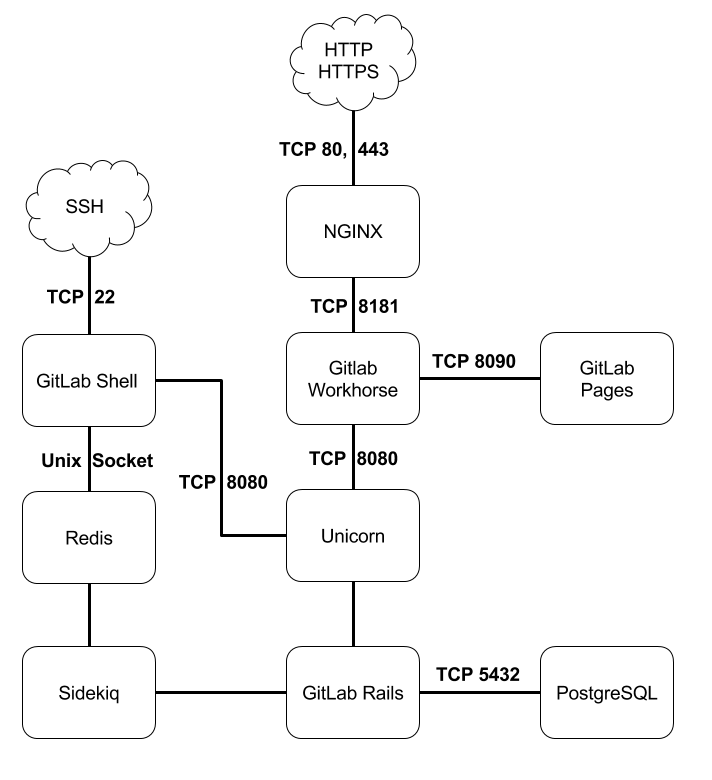
\includegraphics[scale=0.47]{images/gitlab_architecture_diagram.png}
  \caption{Arquitetura do \emph{GitLab}.}
\end{figure}

% ---------------------------------------------------------------
\newpage
\subsection{A arquitetura vista como um escritório físico}

Toda a estrutura do \emph{GitLab} pode ser comparada como um escritório físico. Vejamos alguns componentes na seguinte lista.

\begin{itemize}
    \item \textbf{Os repositórios} serão os bens que o \emph{GitLab} gere. Estes armazenam as chamadas \textit{codebases}, \sout{que são constituídas por todo o código que é usado para construir uma aplicação};
    \item \textbf{\emph{Nginx}} pode ser visto como uma secretaria, onde os utilizadores se dirigem para requisitar certas operações, que serão realizadas pelos funcionários que lá trabalham;
    \item \textbf{Armazenamento de dados} consiste numa série de armários que contêm ficheiros com informações sobre:
    \begin{itemize}
        \item os bens que são armazenados;
        \item os utilizadores que se dirigem à secretaria.
    \end{itemize}
    \item \textbf{\emph{Redis}} é visto como uma espécie de quadro, que contém uma série de tarefas, para serem executadas pelos funcionários;
    \item \textbf{\emph{Sidekiq}} \sout{recolhe tarefas do quadro (\emph{Redis}), tratando principalmente do envio de emails};
    \item \textbf{\emph{Unicorn worker}} é um operário que trata de tarefas rápidas/gerais, coletadas pelo quadro (Redis). Estas consistem principalmente em:
    \begin{itemize}
        \item verificar as permissões dos utilizadores , confirmando a sessão de cada um no \emph{Redis};
        \item criar tarefas para o \emph{Sidekiq};
        \item recolher dados presentes no armazenamento de dados.
    \end{itemize}
    \item \textbf{\emph{GitLab-shell}} pode ser visto também como um funcionário que recebe ordens (por \emph{SSH}), \sout{comunica com o \emph{Sidekiq} por via do \emph{Redis}};
    \item \textbf{\emph{Gitaly}} corresponde a uma espécie de escritório secundário que gere todas as operações feitas através do \emph{git}, desde monitorizar a sua eficiência, até manter cópias dos resultados de operações mais custosas.
\end{itemize}

Com esta simples introdução aos componentes da arquitetura do \emph{GitLab}, conseguimos visualizar o seu funcionamento.

Nas secções a seguir, serão descritos todos os componentes presentes na arquitetura do \emph{GitLab}.


% ---------------------------------------------------------------
\subsection{\emph{GitLab frontend}}

A aplicação \emph{GitLab} apresenta uma interface \emph{web} que utiliza várias tecnologias \emph{open source}. A sua aplicação \emph{web} foi desenvolvida utilizando a \emph{framework} \emph{Ruby on Rails}, baseada num padrão \emph{MVC}. Esta aplicação permite não só, a gestão de repositórios \emph{git}, como também a gestão de comentários que complementam os diferentes projectos.

Relativamente à estruturação da aplicação \emph{web}, é importante destacarmos os seguintes componentes da camada aplicacional:

\begin{itemize}
    \item \emph{\textbf{NGINX}}: é um servidor \emph{web} utilizado para servir conteúdo \emph{web} aos clientes;
    \item \emph{\textbf{GitLab Shell}} e \emph{\textbf{GitLab Workhorse}}: lidam com os comandos \emph{git} enviados pela a aplicação \emph{web}. Ou seja, comandos como \emph{clone, fork, push} ou \emph{pull}, são redirecionados para um destes componentes onde serão executados;
    \item \emph{\textbf{Sidekiq}} e \emph{\textbf{Unicorn}}: utilizados sobretudo para lidarem com a gestão do processamento \emph{Ruby} e pedidos específicos \emph{http}. Estes componentes são completamente \emph{stateless}, pois não persistem qualquer tipo de dados, no entanto são eles que lidam com a gestão de tarefas. Estes componentes são de elevada importância, uma vez que não devem ser apresentados dados inconsistentes na existência de várias instâncias da camada \emph{frontend}.
\end{itemize}

Os componentes descritos em cima fazem parte da camada aplicacional \emph{GitLab}, no entanto, não traduzem a verdadeira essência da aplicação \emph{GitLab}. Isto é, a aplicação ou várias instâncias desta não guardam qualquer tipo de informação a longo prazo. O \emph{frontend} do \emph{GitLab} faz pedidos à camada lógica da aplicação para que possa ser guardado um dado estado ou informação num dos outros componentes da \emph{stack}. O único estado que é guardado na aplicação, é o ficheiro de configuração que abordaremos mais à frente.

\subsubsection{\emph{HAProxy}}

% Tal como foi referido no início da secção \pageref{arq}, o \emph{GitLab} foi desenhado com o intuito de tornar a sua aplicação e os seus serviços altamente disponíveis ao público alvo.

O \emph{HAProxy} (\emph{High Performance TCP/HTTP Load Balancer}) é um servidor \emph{proxy} para \emph{web} que oferece soluções fiáveis como: alta escalabilidade, balanceamento de carga e \emph{proxying} para aplicações que usam \emph{TCP} e \emph{HTTP}.

No contexto da aplicação \emph{GitLab}, o \emph{HAProxy} funciona como um \emph{gateway} que distribui tráfego e pedidos pelos vários servidores que correm a aplicação \emph{GitLab}. Em baixo, encontra-se uma imagem que pretende demonstrar o funcionamento do \emph{HAProxy}, destacado como \emph{load balancer} que recebe vários pedidos \emph{TCP} e \emph{HTTP} e encaminha-os para os servidores que correm o \emph{GitLab}.

\begin{figure}[H]
  \centering
  \includegraphics[scale=0.25]{images/haproxy.png}
  \caption{Exemplo de funcionamento do \emph{HAProxy}.}
\end{figure}

\newpage
"HAProxy will be used as the load balancer for the GitLab frontend. However, it will be a separate load balancer from the one used in the previous HA components. This adds security by having a separation of the outside and inside networks. The HAProxy for GitLab will have its outside requests coming from outside the private network, and forward all its requests to the inside network. By having HAProxy act as the edge node between networks, there is a tight control of what can be accessed on the GitLab frontend machines. No one can try and connect to any unauthorized ports on GitLab, because the HAProxy will only forward specifically allowed requests."

% Relativamente à comunicação entre os vários servidores \emph{proxy} e os servidores aplicacionais, existem três formas distintas: os servidores aplicacionais detêm o seu próprio \emph{SSL} (um distinto para cada servidor);
% https://docs.gitlab.com/ee/administration/high_availability/load_balancer.html

\subsubsection{\emph{Keepalived}}

Juntamente com o \emph{HAProxy}, existe a aplicação \emph{Keepalived} que garante que o serviço \emph{GitLab} está sempre disponivel. Isto é, permanece ativas duas instâncias idênticas do \emph{HAProxy}, garantido assim, que pelo menos uma delas se encontra configurada para um determinado IP, tornando o \emph{HAProxy} eficiente. Se uma instância falhar, outra é automaticamente configurada para o IP anterior (único).



\subsection{\emph{Redis}}

O \emph{Redis} funciona como uma estrutura de armazenamento de dados guardada em memória. É geralmente utilizado para fazer \emph{caching} de dados que, na maioria das vezes, permanecem em memória num curto período de tempo.

Dentro da camada aplicacional do \emph{GitLab}, o \emph{Redis} funciona como um serviço que guarda as sessões ativas de utilizadores e uma lista de tarefas a serem realizadas pelo \emph{Sidekiq}. Isto é, a informação da sessão de um utilizador e as tarefas que estão a ser executadas são guardadas numa ou várias instâncias \emph{Redis}.

Para além destas funcionalidades, o \emph{Redis} permite que os restantes componentes da camada aplicacional guardem o seu estado e o partilhem com o resto dos componentes, por exemplo, através de trocas de messagens. Tal como alguns dos componentes anteriores, é também importante que toda a informação seja consistente e facilmente partilhada com as várias instâncias do \emph{GitLab}. Deste modo, o \emph{Redis} é uma peça fundamental para o funcionamento do \emph{GitLab frontend}.

\subsubsection{\emph{Redis Sentinel}}

O \emph{Redis Sentinel} tem uma funcionalidade muito semelhante ao \emph{Keepalived}. Para garantirmos uma alta disponibilidade, é necessário que para além de existir um \emph{Master} e um \emph{Slave} do \emph{Redis}, exista algo à escuta de falhas de instâncias \emph{Redis}, começando automaticamente o processo de \emph{failover}, que consiste em atribuir uma nova instância.

Com o \emph{Redis Sentinel}, consegue-se garantir a existência e disponibilidade de uma instância \emph{Redis} para um cliente, tornando abstratas todas as falhas.




\subsection{Base de dados - \emph{PostgreSQL}}
O \emph{Postegres} é um sistema de base de dados relacional \emph{open source} que permite o controlo e  persistência de dados.

Os dados que são armazenados incluem dados do utilizador (como \emph{username}, \emph{email}, \emph{password}, definições de conta, etc), permissões dos repositórios, comentários, problemas encontrados e todos os outros dados que não são diretamente controlados pelo \emph{git}. Todos os dados devem, uma vez mais, estar disponíveis e consistentes para poderem ser exibidos e validados corretamente para a aplicação \emph{web} do \emph{GitLab}.


\subsubsection{\emph{Patroni}}

Fazer


\subsection{Gestor de ficheiros distribuído}
Todas as instâncias do \emph{GitLab} que necessitam de acesso ao mesmo sistema de ficheiros, utilizam o \emph{git}. O \emph{git} é um software de gestão e controlo de versões, direcionado principalmente para código fonte, cujo protocolo funciona guardando ficheiros num sistema de ficheiros partilhado.

No entanto, existem também algumas outras pastas que são partilhadas fora do \emph{git}. Incluem-se: a pasta que armazena as chaves \emph{SSH}, recursos estáticos que são carregadps (como é o de imagens) e outros ficheiros que necessitam de estar presentes em todas as instâncias do \emph{GitLab}.


\subsubsection{\emph{ETCD}}

Fazer








% ---------------------------------------------------------------
\newpage
\section{Ficheiros de configuração}

O ficheiro de configuração existente na aplicação \emph{GitLab}, permite indicar e "apontar" os diferentes componentes que permitem a alta disponibilidade e escalabilidade da aplicação. Além disso, este ficheiro contém ainda alguma informação referente ao seu \emph{IP} e ao \emph{hostname} da máquina.

\begin{minted}[bgcolor=bg, 
               fontsize=\footnotesize, 
               framesep=2mm,
               linenos,
               breaklines,
               breakautoindent=true,
               breaksymbolleft=\raisebox{0.8ex}{\tiny\hookrightarrow},
               breaksymbolindentleft=0pt,
               breaksymbolsepleft=1pt,
               breaksymbolright=\raisebox{0.8ex}{\tiny\hookleftarrow},
               breaksymbolindentright=0pt,
               breaksymbolsepright=1pt
]{text}
/etc/gitlab/gitlab.rb
\end{minted}

Através deste ficheiro de configuração 

Identificar os ficheiros onde são alterados valores para comunicar com diferentes componentes ou camadas aplicacionais, por exemplo base da dados.
Usar o mint para colocar partes do texto de configuração.

\begin{minted}[bgcolor=bg, 
               fontsize=\footnotesize, 
               framesep=2mm,
               linenos,
               breaklines,
               breakautoindent=true,
               breaksymbolleft=\raisebox{0.8ex}{\tiny\hookrightarrow},
               breaksymbolindentleft=0pt,
               breaksymbolsepleft=1pt,
               breaksymbolright=\raisebox{0.8ex}{\tiny\hookleftarrow},
               breaksymbolindentright=0pt,
               breaksymbolsepright=1pt
]{text}
/home/git/gitlab/log/
\end{minted}








% ---------------------------------------------------------------
\newpage
\section{Componentes críticos}

Através da análise da arquitetura do \emph{GitLab}, conseguimos detetar facilmente, os componentes que garantem a alta disponibilidade da aplicação que, sem os quais, tornariam o seu desempenho critico e indesejável.

\begin{center}
    \small
    \begin{tabular}{ | l | p{6cm} | p{6cm} |}
    \hline
    \textbf{Componente} & \textbf{Motivo} & \textbf{Solução} \\ \hline
    \textit{HAProxy} & Utilizado para balancear tráfego entre os diferentes componentes como o PostgreSQL ou pedidos como o Redis. & Pag 21. \\ \hline
    \textit{HAProxy} & Utilizado para balancear tráfego entre os diferentes componentes como o PostgreSQL ou pedidos como o Redis. & pag 21. \\
    \hline
    \end{tabular}
\end{center}

\section{Diferentes cenários}
\subsection{Pequena escala}
\subsection{Grande escala}




% ---------------------------------------------------------------
\newpage
\section{Conclusão}

A arquitetura do \emph{GitLab} está dividia em diferentes componentes que fazem do \emph{GitLab} uma aplicação bastante disponível ao utilizador. Esta arquitetura é facilmente relacionada a um sistema distribuído bastante complexo onde existem componentes que podem ser reutilizados no âmbito de outra aplicação.

% ---------------------------------------------------------------
\newpage
\section{Referências}

\vspace{1.3cm}
Bertsche, Ryan. IBM Corp. (2017). GitLab: Highly Available Architecture.

\bigbreak
GitLab Architecture Overview, GitLab Documentation. Acedido em \today, em \url{https://goo.gl/thmr2N} e \url{https://goo.gl/iyR4zN} 

\bigbreak
GitLab High Availability, GitLab Documentation. Acedido em \today, em \url{https://goo.gl/Dt93fF}















% ---------------------------------------------------------------
% DO NOT DELETE
% ---------------------------------------------------------------
\iffalse
\newpage
\section{Troubleshooting}

Para permitir a análise de erros ocorridos na aplicação são armazenadas as alterações feitas nos seus componentes através de ficheiros de log.
% ---------------------------------------------------------------
\newpage

\section{Software Delivery}
\subsection{Definição}
Software Delivery é o processo de fazer chegar um produto a um mercado. Assim, entende-se que poderá ter várias conotações, poderá ser um produto em estado de desenvolvimento alpha a ser entregue a um comprador antes do software estar disponivel à restante comunidade, um update a software interno de uma empresa, ou então a disponibilidade para download de software a toda a comunidade.
Por consequência, pode-se concluir que qualquer pessoa que detenha um produto de software com intenções de venda, desenvolvimento ou mesmo teste e validação de software por questões de qualidade, estará diretamente relacionada com Software Delivery.

\subsection{Estado da Arte}
Antigamente, o desenvolvimento de software era feito com um longo prazo de planeamento e os ciclos de entrega de um produto (quer a disponibilização da versão release assim como updates) eram bastante longos. Atualmente, numa sociedade em que a tecnologia rege o quotidiano da maior parte das pessoas e em que a competição pela atenção dos clientes é enorme, as empresas de software foram obrigadas a mudar os seus protocolos, fazendo com que a entrega de software se torna-se mais dinâmica, frequente e com ciclos de entrega muito curtos de forma a que esta, consiga superar os seus competidores tornando-se mais próxima dos clientes e responder às suas necessidades o mais prontamente possível. Assim, não só os prazos de entrega se tornaram num dos principais fatores de satisfação por parte dos clientes, como também a necessidade do software disponibilizado ser de qualidade, para poder corresponder às expectativas deste.
\par Em suma, a informatização da sociedade obrigou a uma maior necessidade de velocidade e qualidade no que toca a software delivery, o que exigiu com que as empresas de desenvolvimento de software ganhassem grande relevância no dia a dia e que adotassem novas estratégias para conseguir satisfazer os consumidores finais. 

\subsection{GitLab Software Delivery}
Atualmente existem dois tipos de distribuições do GitLab, a versão CE (Community Edition) e a versão EE (Enterprise Edition). 

\subsubsection{Community Edition}
A versão Community Edition é open source não havendo qualquer empresa externa envolvida no processo de delivery ou deployment. A existencia de controlo de versões, revisão de problemas, revisão de código,etc. e a possibilidade de a instalação do sistema poder ser feita em qualquer server, container ou cloud provider destaca o GitLab da concorrência sendo este uma das principais ferramentas utiizadas atualmente por profissionais na àrea da informática por todo o mundo.

\subsubsection{Enterprise Edition}
A versão Enterprise inclui vários pacotes de serviços com diferentes preçarios anuais que incluem desde suporte técnico especializado 24/7 até ferramentas de estatistica, performance, segurança e comunicação via chat.

\subsubsection{Novas versões}
Novas versões do gitlab são disponibilizadas no master branch enquanto que, versões mais antigas e consideradas estáveis são guardadas em branches. De notar que tanto  a EE como a CE necessitam dos add-ons (gitlab-shell e gitaly) que se podem encontrar no master branche.
\fi
% ---------------------------------------------------------------
% ---------------------------------------------------------------
\end{document}
